\documentclass[tikz,border=10pt]{standalone}
\usepackage{tikz}
\usetikzlibrary{shapes,positioning,calc}

\definecolor{garnet}{HTML}{73000A}
\definecolor{atlantic}{HTML}{466A9F}
\definecolor{congaree}{HTML}{1F414D}
\definecolor{warmgrey}{HTML}{676156}
\definecolor{horseshoe}{HTML}{65780B}
\definecolor{rose}{HTML}{CC2E40}
\definecolor{bk70}{HTML}{5C5C5C}

\begin{document}

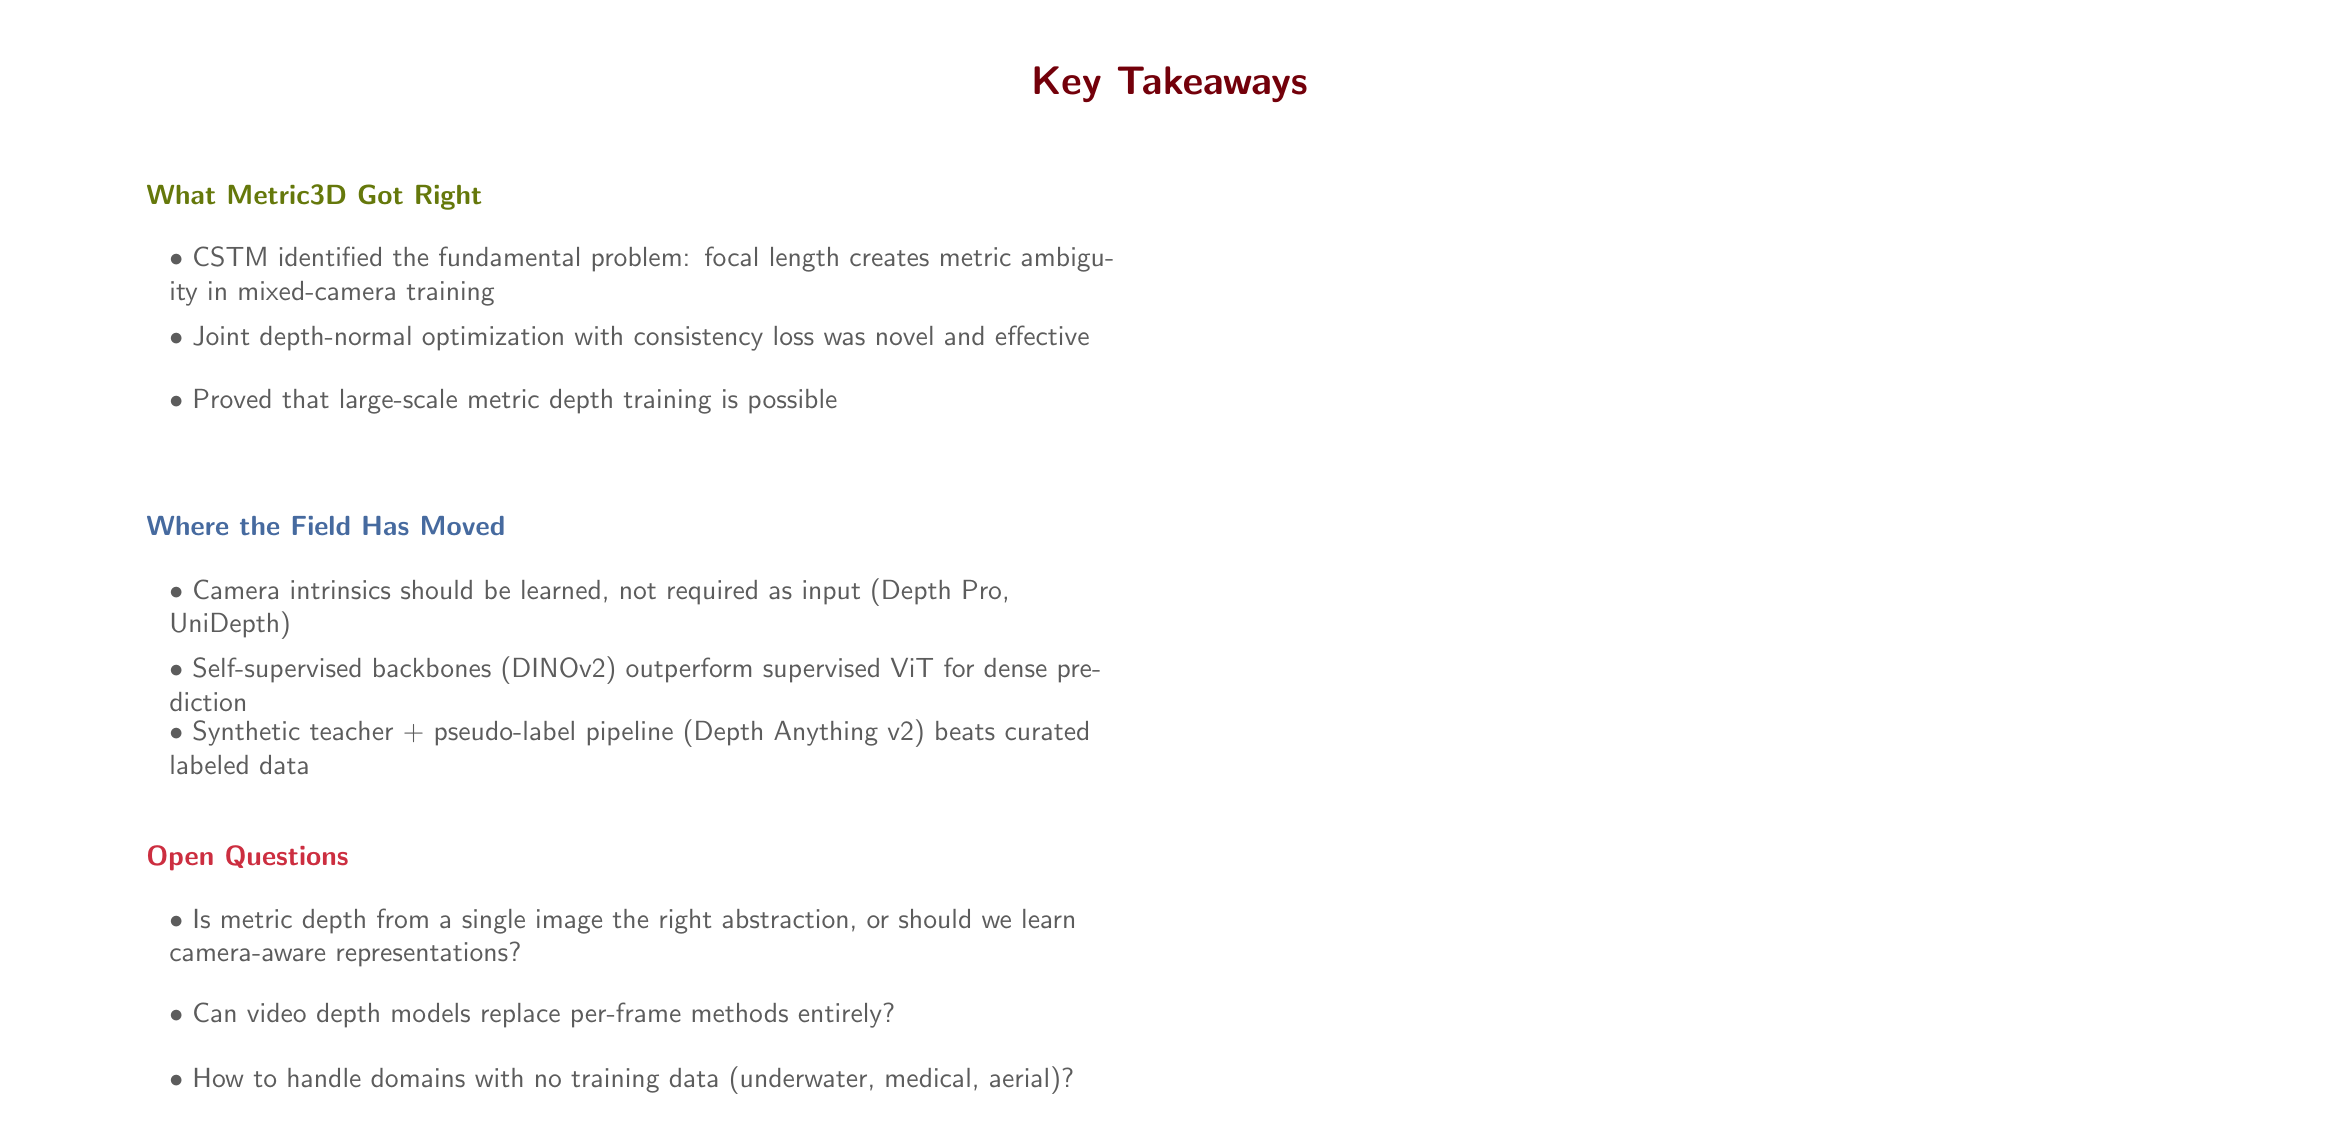
\begin{tikzpicture}[node distance=0pt]

  % Set default font
  \tikzset{every node/.style={font=\sffamily}}

  % Title
  \node[
    anchor=north,
    text width=28cm,
    align=center,
    font=\sffamily\bfseries\Large,
    text=garnet,
    inner sep=0.5cm
  ] (title) at (14cm, 20cm) {Key Takeaways};

  % Section 1: What Metric3D Got Right
  \node[
    anchor=north west,
    align=left,
    font=\sffamily\bfseries\normalsize,
    text=horseshoe,
    inner sep=0cm
  ] (sec1_title) at (1cm, 18cm) {What Metric3D Got Right};

  \node[
    anchor=north west,
    align=left,
    text width=12cm,
    font=\sffamily\normalsize,
    text=bk70,
    inner sep=0cm,
    line width=0pt
  ] (sec1_bullet1) at (1.3cm, 17.2cm) {$\bullet$ CSTM identified the fundamental problem: focal length creates metric ambiguity in mixed-camera training};

  \node[
    anchor=north west,
    align=left,
    text width=12cm,
    font=\sffamily\normalsize,
    text=bk70,
    inner sep=0cm,
    line width=0pt
  ] (sec1_bullet2) at (1.3cm, 16.2cm) {$\bullet$ Joint depth-normal optimization with consistency loss was novel and effective};

  \node[
    anchor=north west,
    align=left,
    text width=12cm,
    font=\sffamily\normalsize,
    text=bk70,
    inner sep=0cm,
    line width=0pt
  ] (sec1_bullet3) at (1.3cm, 15.4cm) {$\bullet$ Proved that large-scale metric depth training is possible};

  % Section 2: Where the Field Has Moved
  \node[
    anchor=north west,
    align=left,
    font=\sffamily\bfseries\normalsize,
    text=atlantic,
    inner sep=0cm
  ] (sec2_title) at (1cm, 13.8cm) {Where the Field Has Moved};

  \node[
    anchor=north west,
    align=left,
    text width=12cm,
    font=\sffamily\normalsize,
    text=bk70,
    inner sep=0cm,
    line width=0pt
  ] (sec2_bullet1) at (1.3cm, 13cm) {$\bullet$ Camera intrinsics should be learned, not required as input (Depth Pro, UniDepth)};

  \node[
    anchor=north west,
    align=left,
    text width=12cm,
    font=\sffamily\normalsize,
    text=bk70,
    inner sep=0cm,
    line width=0pt
  ] (sec2_bullet2) at (1.3cm, 12cm) {$\bullet$ Self-supervised backbones (DINOv2) outperform supervised ViT for dense prediction};

  \node[
    anchor=north west,
    align=left,
    text width=12cm,
    font=\sffamily\normalsize,
    text=bk70,
    inner sep=0cm,
    line width=0pt
  ] (sec2_bullet3) at (1.3cm, 11.2cm) {$\bullet$ Synthetic teacher + pseudo-label pipeline (Depth Anything v2) beats curated labeled data};

  % Section 3: Open Questions
  \node[
    anchor=north west,
    align=left,
    font=\sffamily\bfseries\normalsize,
    text=rose,
    inner sep=0cm
  ] (sec3_title) at (1cm, 9.6cm) {Open Questions};

  \node[
    anchor=north west,
    align=left,
    text width=12cm,
    font=\sffamily\normalsize,
    text=bk70,
    inner sep=0cm,
    line width=0pt
  ] (sec3_bullet1) at (1.3cm, 8.8cm) {$\bullet$ Is metric depth from a single image the right abstraction, or should we learn camera-aware representations?};

  \node[
    anchor=north west,
    align=left,
    text width=12cm,
    font=\sffamily\normalsize,
    text=bk70,
    inner sep=0cm,
    line width=0pt
  ] (sec3_bullet2) at (1.3cm, 7.6cm) {$\bullet$ Can video depth models replace per-frame methods entirely?};

  \node[
    anchor=north west,
    align=left,
    text width=12cm,
    font=\sffamily\normalsize,
    text=bk70,
    inner sep=0cm,
    line width=0pt
  ] (sec3_bullet3) at (1.3cm, 6.8cm) {$\bullet$ How to handle domains with no training data (underwater, medical, aerial)?};

\end{tikzpicture}

\end{document}
